 \documentclass[10pt,a4paper]{article}
\usepackage[utf8]{inputenc}
%\usepackage{fontspec} % This line only for XeLaTeX and LuaLaTeX
\usepackage{pgfplots}
\usepackage{pgf}
\usepackage[english]{babel}
\usepackage{amsmath}
\usepackage{amsfonts}
\usepackage{amssymb}
\usepackage{graphicx}
\graphicspath{ {../figures/} }
%\usepackage{svg}
\usepackage{color,soul}
\usepackage{listings}
\usepackage{setspace}
\title{\textsf{\textbf{Droplet Electro-Bouncing in Low-Gravity}}}
\vspace{-25mm}
\author{Erin S. Schmidt, Mark M. Weislogel}
\date{}

\usepackage{abstract}
\renewcommand{\abstractnamefont}{\normalfont\bfseries}
\renewcommand{\abstracttextfont}{\normalfont\small\itshape}

\usepackage{setspace}
\newlength\figureheight
\newlength\figurewidth
\setlength\figureheight{7cm}
\setlength\figurewidth{10cm}

\usepackage[
backend=biber,
style=phys,
sorting=none
]{biblatex}
\addbibresource{thesis.bib}

\begin{document}
\maketitle
\doublespacing

\begin{abstract}
\noindent
We investigate the dynamics of spontaneous jumps of water droplets from electrically charged superhydrophobic dielectric surfaces during a sudden step reduction in gravity level. In the brief free-fall environment of a drop tower, with a non-homogeneous external electric field (with strengths ~0.39-2.36 kV/cm) arising due to dielectric surface charges, body forces acting on the jumped droplets are primarily supplied by polarization stress and Coulombic attraction instead of gravity. This electric body force leads to a droplet bouncing behavior similar to well-known phenomena in 1-g, though occurring for much larger droplets ($\sim$ 0.5 mL). We show a simple model for the phenomenon, its scaling, and asymptotic estimates for droplet time of flight. The droplet net charge, estimated to be on the order of 1E-9 C, is field induced rather than by contact charging at the (PTFE coated) hydrophobic interface. In 1-g, for Weber numbers $>$ 0.4, impact recoil behavior on a super-hydrophobic surface is normally dominated by damping from contact line hysteresis. However, at the low Bond and Ohnesorge numbers occurring in free-fall, the droplet impact dynamics additionally include electrohydrodynamic surface wettability effects. This is qualitatively discussed in terms of trends in coefficients of restitution and dimensionless contact time.
\end{abstract}

\newpage
\section{Introduction}
\begin{quote}
``When the influence of gravity on fluid behavior is diminished or removed, other forces, otherwise of small significance, can assume paramount roles.''
- NRC Report to NASA, 2003  \cite{motil_priorities_2012}
\end{quote}

Our terrestrially born intuition about how liquids flow is easily confounded in a low-gravity environment. This should come as little surprise, as we are creatures evolved at the bottom of a steep gravity well; gravity is natural to us. However when the magnitude of the gravity body-force becomes small, other forces come into play in fluid dynamics which are otherwise negligible, relatively speaking, under normal circumstances in 1-g. This 1-g cognitive bias leads to a plethora of problems which are both trivially easy to solve in 1-g, and which despite decades of study continue to elude solutions in a low-gravity context. One example of these problems is the so-called ``phase separation'' problem of separating a gas phase from a multi-phase flow (or the reverse case) without the aid of gravitational buoyancy. Sans buoyancy otherwise mundane activities such as venting a gas or settling a liquid in a tank become problematic \cite{petrash_controlling_1964}. Trapped bubbles can vapor lock ECLSS (Environmental Control and Life Support), power, or propulsion systems \cite{jenson_passive_2014}. Issues of phase separation have so bedeviled human endeavors in space that an entire Apollo Saturn 1B mission (AS-203) was earmarked to study them \cite{hastings_[saturn_1965}. This problem has for some time motivated a quest for substitute body forces, and the present work follows in that august tradition.

Considering the scope of this problem of poor low-gravity intuition, we would profit by identifying a scale to quantify how wrong our intuition is. First, let's clear up a common misnomer about the state of ``zero-gravity''. The theory of general relativity is based on the fundimental equivalence of gravity and acceleration. There is no known way to determine whether one is in gravity-free space or free-falling in a gravitational field (or conversely whether or not we are uniformly accelerating, or standing at rest in a gravitational field). This is sometimes called the equivalence principle of general relativity (e.g. the equivilence of gravitational and inertial mass). In theoretical terms a zero-g experiment performed in a drop tower on the surface of the Earth is equivalent to the same experiment performed in the nearly gravity-free deep space between galaxies, despite the fact that the drop tower itself is in a 1-g gravity field. At the orbital altitude of the Internation Space Station (ISS) the gravity level is still nearly 90\% of its value at sea-level on Earth, but the astronauts aboard ISS feel weightlessness because they are free-falling. In a practical sense there is never true zero-g, even in the aforemention dark space between galaxies, as there are always small, but nonetheless, measureable forces to accelerate any body. For instance in low-Earth orbit, accelerations due to drag in the tenuous outer atmosphere are on the order of $1 \times 10^{-6}$ g, hence the term ``microgravity''. This small acceleration provides an ersatz gravity, but there are also other forces present. Foremost of these are capillary forces. 

Capillary forces are due to the cummulative effect of a large number of very short range molecular interations and in a 1-g context are usually quite weak, relatively speaking. However, in a low-gravity environment these are nearly the only forces present, and are therefore strong in a relative sense. In comparing the relative magnitudes of gravity and the unusually strong capillary force we arrive at a useful figure of merit for assesing how wrong our fluid mechanical intuition is likely to be in a low-gravity context. This figure of merit is the Bond number dimensionless group
\[ \mathbb{B}\mbox{o} \equiv \frac{g R^2 \Delta \rho}{\gamma} 
\]
where $g$ is the acceleration, $R$ is the interfacial radius of curvature, $\Delta \rho$ is the difference in densities across the interface (which simplifies to $\rho$, for large $\Delta \rho$, as in the case of a air-water interface), and where $\gamma$ is the surface tension. In cases where $\mathbb{B}\mbox{o}$ is small, a liquid is effectivly in low-gravity regardless of the nominal local gravity level. Very small droplets ($R < 1$ mm), for instance, are in low-gravity for all intents and purposes and have nearly spherical shapes. Contrarily, in a space environment in cases where $R$ becomes large, such as with the case of large diameter spacecraft propellant tanks then $ \mathbb{B}\mbox{o} \gg 1$ even though the acceleration is small. As a corrallary to this discussion we note that on the basis of dimensional similarity, we can accurately simulate the low-gravity fluid mechanics of large propellant tanks even in small drop towers simply by scaling dimensonless groups like the Bond number. 

As with surface tension, electrostatic forces also have useful applications as substitutes for gravity. Electrohydrodynamic (EHD) body forces have been suggested to combat thermal stratification of propellants under low-g conditions where bouyancy induced natural convection is very small \cite{blackmon_collection_1965}. In this case electro-convection is an analog of natural convection due to a dielectric permitivity gradient (as opposed to a fluid density gradient), which is a function of fluid temperature, in the presence of a body force field (in this case an electric field). The study also suggested applications in cryogenic tank vent screening, and in reducing heat transfer to cryogenic propellants (and thus boiloff losses) by dielectrophoretically positioning ullage vapors around the tank walls as a thermal barrier. EHD forces have been studied for enhancing boiling heat transfer by promotion of bubble detachment and prevention of dryout (again as an ersatz bouyancy) \cite{snyder_dielectrophoresis_2001} \cite{di_marco_influence_2003} \cite{marco_use_2012}. EHD heat pipes, which substitute an electrode structure for the capillary wicking structure of a conventional thermocapillary heat pipe can evade the wicking limit \cite{jones_electrohydrodynamic_1973}. These are restricted to the use of insulating dielectric liquids (which usually have relatively low thermal conductivity), but are highly robust against dryout, support active flow control, and have low viscous losses. Dielectrophoretic settling of cryogenic propellants (in both total and partial communication configurations), has been studied analytically in both static \cite{hurwitz_electrohydrodynamic_1966} and dynamic cases \cite{koval_dynamics_1967}, and in drop tower experiments \cite{fax_dielectrophoretic_1969}. EHD forces have also beeen suggested for low-g slosh baffling \cite{boretz_orbital_1970} \cite{petrash_use_1968} \cite{hurwitz_dielectrophoretic_1968}, and studied extensively for the mitigation of vapor pullthrough during tank emptying (and concomittent minimization of propellant residuals at burnout) in a series of experiments at the NASA Lewis (now Glenn) Research Center 2.2 s drop tower facillity \cite{berenyi_dielectrophoretic_1970}. 

\subsection{Spontaneous Droplet Jump}
Low-gravity droplet dynamics, and the dynamics and applications of the so-called spontaneous droplet jump, is an active area of study at the Portland State University Dryen Drop Tower labratory (DDT). When a nonwetting, gravity dominated sessile droplet (e.g. a puddle), initially at rest in the Cassie-Baxter state undergoes a large step reduction in $\mathbb{B}\mbox{o}$ it will spontaneously jump away from the surface. The Cassie-Baxter state is a metastable non-wetting state on a textured surface, sometimes also known as the Fakir state. This was first observed experimentally by Kirko \emph{et al.} \cite{kirko_phenomenon_1970} in 1970 and later by Wollman \emph{et al.} in 2006 in a set of experiments conducted using a low-gravity drop tower \cite{wollman_more_2016}. The kinetic energy of the jump is supplied by the defect in free surface energy as the new minimum energy surface equilibrium has approximately constant curvature. If the viscous energy losses by shear, and internal flows during roll up are neglected, as well as energy lost due to the hysteresis of the dynamic contact line, then the available kinetic energy is given by
\[KE = SE_2 -SE_1 = [(\sigma A)_{gl} + (\sigma A)_{sg}]_2 - [(\sigma A)_{ls} + (\sigma A)_{gl} + (\sigma A)_{sg}]_1. \]

The droplet `rolls up' as it jumps away from the surface due to radial motion of a capillary wave away from the contact line. The characteristic time scale of the rolling up scales as $t_j \sim R_p/U ~(\rho H R^2_p/\sigma)^{1/2}$ \cite{attari_puddle_2016}, which resembles the contact time, $\tau \approx 2.6(\rho R^3_d/\sigma)^{1/2}$ reported by Richard \emph{et al.} in 2002 for the related problem of droplets impacting hydrophobic surfaces in 1-g \cite{richard_surface_2002}. For droplets with radial symmetry and sufficiently high initial $\mathbb{B}\mbox{o}$ these waves coalesce as a shock leading to geysering and creation of satellite drops by the Rayleigh-Plateau breakup of the geyser. In the case of smaller jumping droplets, the capillary waves do not lead to geysering, and are viscously damped to varying degrees during the brief free-fall period of the drop tower.

The spontaneous droplet jump phenomenon provides a useful window though which to study the dynamics of large-length scale capillary dominated droplets. The physics of such massive droplets (far beyond the 1-g millimetric capillary length scale) utterly defy terrestrial expectations about the ways in which liquid droplets `should' behave, and also are of critical practical importance in a space systems setting where large capillary length scale multiphase flows are common.

\subsection{Droplet Electro-bounce}
During `rolling-up' under ideal conditions, the droplet jump phenomenon is governed by a balance of inertia and surface tension forces, and once aloft the droplet motion is nominally in a regime of pure drag, however other forces can again come into play. 

\emph{Occasionally we observe jumped droplets to decelerate and return to the superhydrophobic surface, rebounding multiple times after fashion of a rigid body bouncing on a surface under 1-g. The forces at work in this phenomenon are presumably electrostatic in origin.} This was unintended, but the phenomenon is interesting. Admittedly, there is a certain irony that this typical failure of low-gravity intuition come as any surprise to experienced low-gravity researchers. A time-lapsed composite image showing an example of the phenomenon is shown in Figure \ref{fig:bounce}.  

\newpage
\begin{figure}[htb]
\centering
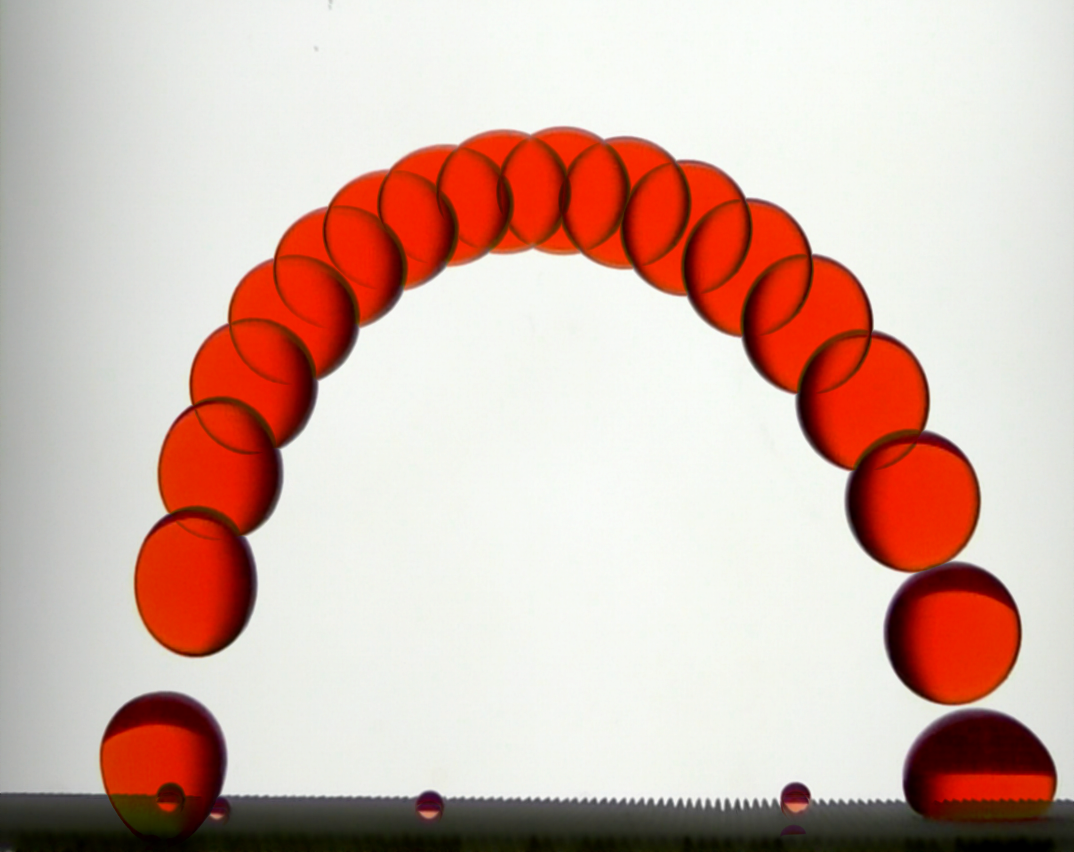
\includegraphics[width=0.75\textwidth]{bounce}
\caption{The trajectory of a $0.5$ mL droplet is captured in a composite image over a single bounce period ($\sim 1.25$ s). The surface potential of the superhydrophobic dielectric is $1.25 \pm 0.41$ kV. \label{fig:bounce}}
\end{figure}

This ``electro-bounce'' phenomenon is the subject of this thesis. We begin with some preliminary observations of the phenomenon:
\begin{itemize}
\item We have observed droplet accelerations on the order of 10's of cm/s$^2$ in proximity to charged surfaces.
\item Droplets appear to be attracted to regions of high electric field. The horizontal (surface plane parallel) components of the droplet trajectory usually oscillate about their initial position during drops (except in cases of nearly pure 1-D vertical translation). For especially small drops close to the spontaneous droplet jump limit ($V_d \sim 0.01$ mL) the droplets do not jump, but translate across the surface in a hovering regime until either they reach a local maximum of the electric field, or until their motion is sufficiently damped by contact line hysteresis that pinning arrests their motion.
\item Droplets appear to have net free charge. In cases of multiple simultaneous droplet jumps the droplets repel each other as they bounce or hover in orbital motion around regions of strong field.
\item The magnitude of the droplet trajectory maxima (apoapses) appear to be related to the droplet volume (which affects their mass, and initial jump velocity, and thence their inertia), and to the electric field strength.
\end{itemize}

There are several potential origins of the electric charge responsible for this phenonenon. It is well known that water acquires free charge (usually positive) when in contact with certain polymers, especially polytetrafluoroethylene (PTFE) \cite{langmuir_surface_1938}, through a process called contact charging. The superhydrophobic surfaces used in the spontanous droplet jump experiments have thin PTFE coatings, and we observe that it is extremely easy to produce significant surface potentials ($\sim 100-500$ V) by simply running streams of filtered water over them. A study of this water on PTFE contact charging phenomenon was done by Yatsuzuka \emph{et al.} \cite{yatsuzuka_electrification_1994}, who suggest this process results from formation of an electrical double layer formed by selective adsoption of ions at the polymer surface. They also found that the specific charge on the droplets in contact with the surface depends on their surface velocity and conductivity. New developments suggest that adsoption of $OH^-$ ions are the source of the double layer \cite{beattie_intrinsic_2006} \cite{strazdaite_water_2015}. This is the most likely accidental source of charge on the suphydrophobic surface. Given the large roughness (in the sense of the ratio projected to actual surface area), of the superhydrophobic surfaces used in the experiment, and given that the droplets are initially in a Cassie-Baxter state, an electrically insulating air layer is maintained that prevents grounding of the droplets despite the large potential difference between them and and the surface charges. Ultimately it is this potential, in the energetic sense, that is responsible for the droplet bouncing motion we observe. 

The source of the net free charge on the droplets is another issue. The droplet charge could also be due to this contact charging mechanism. For instance, in a 1996 paper, NASA flight engineer Don Pettit discusses the problem of flow induced charging of liquids in a low-gravity context, resulting ultimately from contact charging phenomenon \cite{pettit_donald_flow_????}. Another mechanism for the droplet charge is field induced charging. Field induced charging occurs due to physical breakup of a conductor having a field induced dipole. In our case this occurs when the droplet is deposit on the charged surface by a syringe. The metal syringe needle tip, and the liquid in the syrigne itself are essentially a ground connection which is broken when the syringe is removed. Field induced charging is at work in the famous Kevin thunderstorm, and is applied in inkjet, and electrospay technologies (where in each case the breakup is by the Rayleigh-Plateau instability). Notably, in Pettit's discussion of contact charging of liquids in low-g, he remarks on accidental electrostatic ``hula-ing'' of sillicon oil droplets when ejected from a syringe in the vicinity of a highly-charged polymer surface during an experiment conducted aboard STS-5 by mission specialist Joseph Allen. Depending on the (highly-variable) electrical conductivity of the sillicon oil, and the material of the syringe used in the experiment, the charge could as easily be field induced as due to contact charging. Relatedly, in a series of informal, and somewhat whimsical experiments Pettit electrostatically orbited small water droplets around a triboelectrically charged PTFE knitting needle while aboard ISS during expedition 30/31 \cite{stevenson_electrostatic_2015}. Again, in this case, the droplet charge is very likely field induced.  

\subsection{Applications}
Study of the droplet electro-bounce phenomenon may have results which can be extended to useful applications in a space environment.

External surfaces of spacecraft tend to become charged with time due to the space environment itself. Surface charging largely occurs due to low energy electrons (3-50 keV) which do not penetrate the surface of the spacecraft external stucture \cite{czepiela_charging_1997}. This deposited charge accumulates and can lead to significant potential differences between different parts of a spacecraft, sometime leading to breakdown and discharge, called Paschen discharge. Deep dielectric charging occurs when higher energy charged particles penetrate the surface of a dielectric material, which can also lead to large potential differences if the dielectric leakage is lower than the external charging rate. The ultimate sources of these charges are trapped charged particles of the van Allen radiation belts, galactic cosmic rays, and the solar wind. In a fluid mechanical context, this accumulated charge could be problematic during any multiphase venting process, as might be expected to occur during autonomous satellite servicing refueling operations, or during boil-off venting of cryogens stored over long periods in a space environment (as in crewed Mars missions, or in propellant depot operations). Such venting, if uncontrolled, can lead to contamination of spacecraft surfaces by the propellant.

As previously noted, robust phase separation is critical to high reliability multiphase systems used in thermal control and life support. Active (but solid-state) phase seperation for ECLSS multiphase flows, espcially high void-fraction flows is a possible application of this work. Such flows pertain to dish washing, laundry, waste solids drying, food processing, the Sabatier CO$_2$ reaction, and possibly in vapor-compression cycle condensers. Phase seperation for other disperse droplet flows include electrostatic droplet seperators for high-efficiency Rankine-cycle turbines (which require a droplet-free vapor phase entering the turbine, but where convertional superheat approaches comes with severe mass penalties) \cite{unterberg_zero_1962}, or more speculatively, in high temperature liquid droplet radiators with electrostatic collection \cite{white_liquid_1987}. Removal of satellite droplets produced during pippetting in wet-lab research outside of a glovebox environment aboard ISS has also been recently suggested as a application of the work \hl{[ref, personal discussion with NASA MSFC folk at ASGSR17 conference]}. Droplets can become spontaneously charged by contact with standard micropipette tips \cite{choi_spontaneous_2013}, and this free charge can possibly be leveraged for the purposes of phase separation in low-gravity. 

\subsection{Overview of this Thesis}
This work primarily concerns itself with development of a simple model to aid in design of future electrostatic disperse droplet phase separators. To that end this work encompasses:
\begin{enumerate}
\item A simple mathematical model of droplet electro-bounce, its scale analysis, and asymptotic estimates for droplet peak apoapses and times-of-flight.
\item The results of a controlled experiment, where the effect of key independent variables droplet volume $V_d$, and dielectric surface charge density $\sigma$, on droplet trajectories is tested.
\item Science of opportunity comprising experimental data on droplet impacts at very low Weber and Ohnesorge numbers, for varying levels of electrostatic Bond number. 
\end{enumerate}

\printbibliography
\end{document}
